\subsubsection{Optimisation for Deep Learning}

\begin{remark} \hlt{Optimisation}\\
A cost function $J(\bm{\theta})$ is reduced to improve some performance measure $P$.\\
Optimisation algorithms include some specialisation on specific structure of machine learning objective functions.\\
Cost function is average over training set,
\begin{equation}
J(\bm{\theta}) = \mathbb{E}_{(\bm{x}, y) \sim \hat{p}_{\text{data}}} L(f(\bm{x}; \bm{\theta}), y) \nonumber
\end{equation}
where $L$ is per-example loss function, $f(\bm{x}; \bm{\theta})$ is predicted output given input $\bm{x}$, $\hat{p}_{\text{data}}$ is empirical distribution. For supervised learning, $y$ is target output.\\
The goal is to usually to minimise objective function where expectation is taken on data generating distribution $p_{\text{data}}$ rather than over the finite training set:
\begin{equation}
J^*(\bm{\theta}) = \mathbb{E}_{(\bm{x}, y) \sim p_{\text{data}}} L(f(\bm{x}; \bm{\theta}), y) \nonumber
\end{equation}
Note that machine learning algorithm usually minimises a surrogate loss function, and halts when convergence criterion based on early  stopping is satisfied.
\end{remark}

\begin{definition} \hlt{Empirical Risk Minimisation}\\
To minimise expected loss on training set, where $\hat{p}(\bm{x}, y)$ is the empirical distribution. The empirical risk is
\begin{equation}
\mathbb{E}_{\bm{x}, y \sim \hat{p}_{\text{data}}(\bm{x}, y)}[L(f(\bm{x}, \bm{\theta}), y)] = \frac{1}{m} \sum\limits_{i=1}^m L(f(\bm{x}^{(i)}; \bm{\theta}), y^{(i)}) \nonumber
\end{equation}
where $m$ is number of training samples. Note that empirical risk minimisation is prone to overfitting, as models with high capacity may memorise the training set.
\end{definition}

\begin{remark} \hlt{Batch and Minibatch Algorithms}\\
Objective algorithms for machine learning computes each update to the parameters based on expected value of cost function using only a subset of terms of full cost function.\\
For maximum likelihood estimation problems, note that
\begin{align}
\bm{\theta}_{\text{ML}} &= \arg \max_{\bm{\theta}} \sum\limits_{i=1}^m \log p_{\text{model}}(\bm{x}^{(i)}, y^{(i)}; \bm{\theta}) \nonumber \\
J(\bm{\theta}) &= \mathbb{E}_{\bm{x}, y \sim \hat{p}_{\text{data}}} \log p_{\text{model}} (\bm{x}, y; \bm{\theta}) \nonumber
\end{align}
The gradient is then
\begin{equation}
\nabla_{\bm{\theta}} J(\bm{\theta}) = \mathbb{E}_{\bm{x}, y \sim \hat{p}_{\text{data}}} \nabla_{\bm{\theta}} \log \log p_{\text{model}} (\bm{x}, y; \bm{\theta}) \nonumber
\end{equation}
If the optimisation algorithm uses the entire training set, then it is a batch gradient method.\\
If a single sample is used at a time, then this is a stochastic/online gradient method.\\
For algorithms that uses more than one but less than all samples, then this is a minibatch gradient method.
\end{remark}

\begin{remark} \hlt{Challenges: Ill-Conditioning of Hessian Matrix $H$}\\
May cause stochastic gradient descent to be stuck where very small step increases the cost function.\\
Note that a gradient descent step of $- \bm{\epsilon} \bm{g}$ will add
\begin{equation}
\frac{1}{2} \epsilon^2 \bm{g}^T \bm{H} \bm{g} - \epsilon \bm{g}^T \bm{g} \nonumber
\end{equation}
to the cost. This will be a problem when $\frac{1}{2} \epsilon^2 \bm{g}^T \bm{H} \bm{g} > \epsilon \bm{g}^T \bm{g}$.\\
Monitor squared gradient norm $\bm{g}^T \bm{g}$ and $\bm{g}^T \bm{H} \bm{g}$ term. When ill-conditioning happens, gradient norm does not shrink significantly but $\bm{g}^T \bm{H} \bm{g}$ term grows more than order of magnitude, and learning rate shrinks.
\end{remark}

\begin{remark} \hlt{Challenges: Local Minimums}\\
Model is identifiable if a sufficiently large training set can rule out all but one setting of model parameters.\\
There may be an extremely large or uncountably infinite amount of local minima in a cost function. If the local minima have a high cost compared to global minimum, then this is problematic.
\end{remark}

\begin{remark} \hlt{Challenges: Plateaus, Saddle Points, Flat Regions}\\
For a function $f: \R^n \rightarrow \R$, expected ratio of saddle points to local minima grows exponentially with $n$. Hessian matrix at a saddle point has a mixture of positive and negative eigenvalues.\\
Degenerate regions with flat gradient may correspond to high value of objective function.
\end{remark}

\begin{remark} \hlt{Challenges: Cliffs and Exploding Gradients}\\
On extremely steep cliff structure, gradient update step may move parameters extremely far, losing most of the optimisation work done previously. The consequences may be mitigated using gradient clipping heuristics, which reduces the step size to be small enough.
\end{remark}

\begin{remark} \hlt{Challenges: Long-Term Dependencies}\\
Occurs when computational graph becomes very deep. Let a computational graph contain a path that repeatedly multiply a matrix $\bm{W}$. After $t$ steps, this is $\bm{W}^t$. Let the eigen-decomposition of $\bm{W}$ be $\bm{W} = \bm{V} \text{diag}(\bm{\lambda}) \bm{V}^{-1}$. Then we can see that $\bm{W}^t = (\bm{V} \text{diag}(\bm{\lambda}) \bm{V}^{-1})^t = \bm{V} \text{diag}(\lambda)^t \bm{V}^{-1}$.\\
There will be a vanishing and exploding gradient problem if gradients on the graph are scaled according to $\text{diag}(\bm{\lambda})^t$.  Note that recurrent networks uses same $\bm{W}$ at each time step, hence may face the problem.
\end{remark}

\begin{figure}[H]
\centering
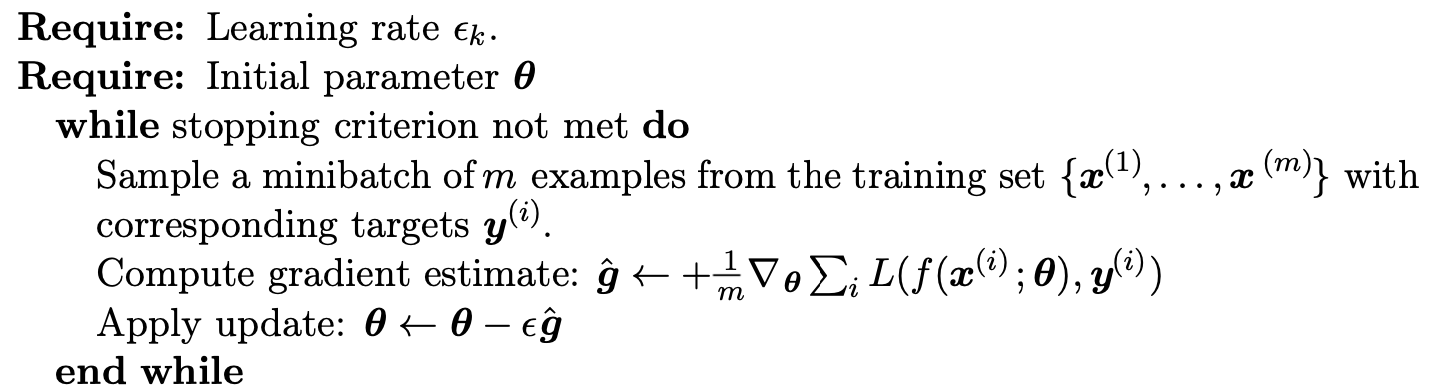
\includegraphics[scale=0.45]{/math/dl/sgd}
\caption{Stochastic Gradient Descent (SGD) update at training iteration $k$}
\end{figure}

\begin{remark} \hlt{Stochastic Gradient Descent (SGD)}\\
Crucial parameter is the learning rate, which may be changed over time; at iteration $k$ this is $\epsilon_k$.\\
The SGD gradient estimation introduces a source of noise that does not vanish even at minimum. A sufficient condition to guarantee converge of SGD is
\begin{equation}
\sum\limits_{k=1}^{\infty} \epsilon_k = \infty, \ \ \ \sum\limits_{k=1}^{\infty} \epsilon_k^2 < \infty \nonumber
\end{equation}
In practice, it is common to decay learning rate linearly until iteration $\tau$:
\begin{equation}
\epsilon_k = (1- \alpha)\epsilon_0 + \alpha \epsilon_{\tau} \nonumber
\end{equation}
where $\alpha = \frac{k}{\tau}$. After iteration $\tau$, leave $\epsilon$ as a constant.\\
Note that SGD computation time per update does not growth with number of training examples.
\end{remark}

\begin{figure}[H]
\centering
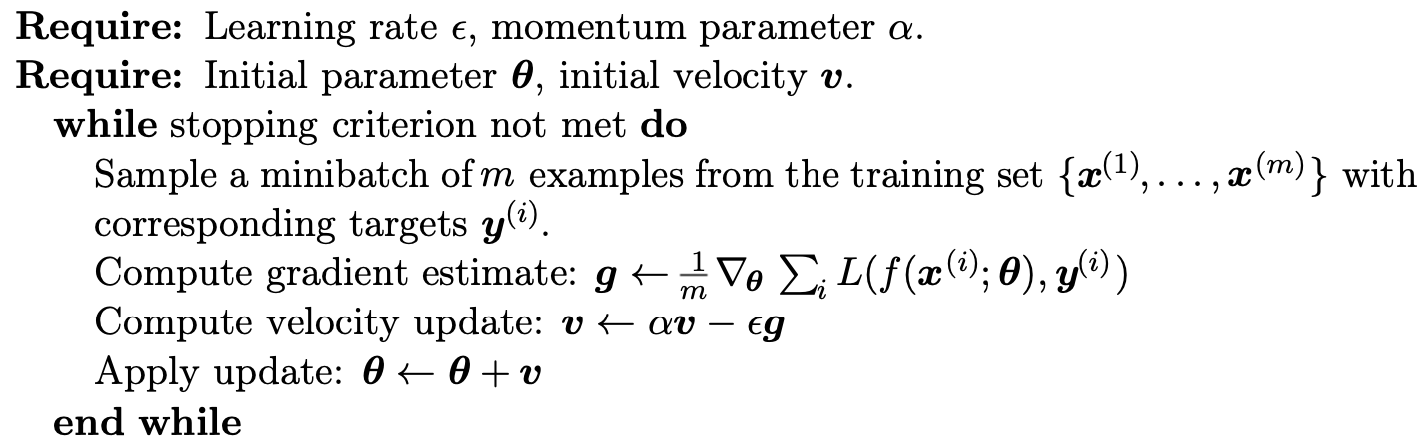
\includegraphics[scale=0.45]{/math/dl/sgdmom}
\caption{Stochastic Gradient Descent (SGD) with momentum}
\end{figure}

\begin{remark} \hlt{Momentum Algorithm}\\
Algorithm introduces variable $\bm{v}$ that is set to an exponentially decaying average of negative gradient.\\
Hyperparameter $\alpha \in [0, 1)$ determines how quickly the contributions of previous gradients exponentially decay.\\
The update rule is given by
\begin{align}
\bm{v} &\leftarrow \alpha \bm{v} - \epsilon \nabla_{\bm{\theta}} \left(\frac{1}{m} \sum\limits_{i=1}^m L(\bm{f}(\bm{x}^{(i)}; \bm{\theta}), \bm{y}^{(i)}) \right) \nonumber \\
\bm{\theta} &\leftarrow \bm{\theta} + \bm{v} \nonumber
\end{align}
The larger $\alpha$ is relative to $\epsilon$, the more previous gradients affect current direction.
\end{remark}

\begin{figure}[H]
\centering
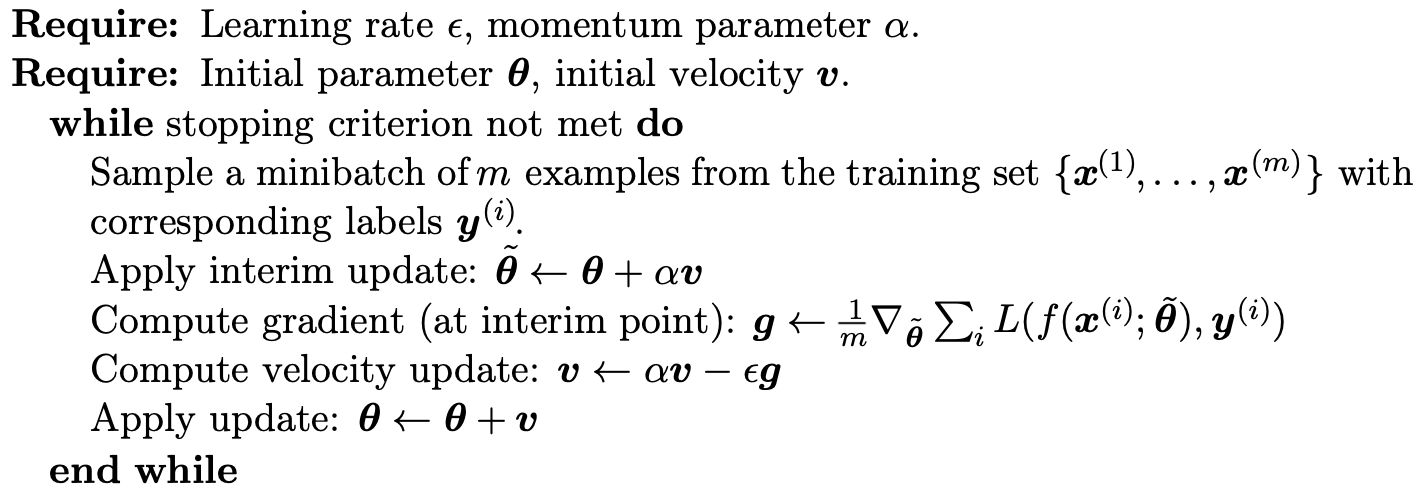
\includegraphics[scale=0.46]{/math/dl/sgdnest}
\caption{Stochastic Gradient Descent (SGD) with Nesterov momentum}
\end{figure}

\begin{remark} \hlt{Nesterov Momentum}\\
Inspired by Nesterov's accelerated gradient method, the update rules are:
\begin{align}
\bm{v} &\leftarrow \alpha \bm{v} - \epsilon \nabla_{\bm{\theta}} \left(\frac{1}{m} \sum\limits_{i=1}^m L(\bm{f}(\bm{x}^{(i)}; \bm{\theta} + \alpha \bm{v}), \bm{y}^{(i)}) \right) \nonumber \\
\bm{\theta} &\leftarrow \bm{\theta} + \bm{v} \nonumber
\end{align}
Note, gradient is evaluated after current velocity is applied.
\end{remark}

\begin{figure}[H]
\centering
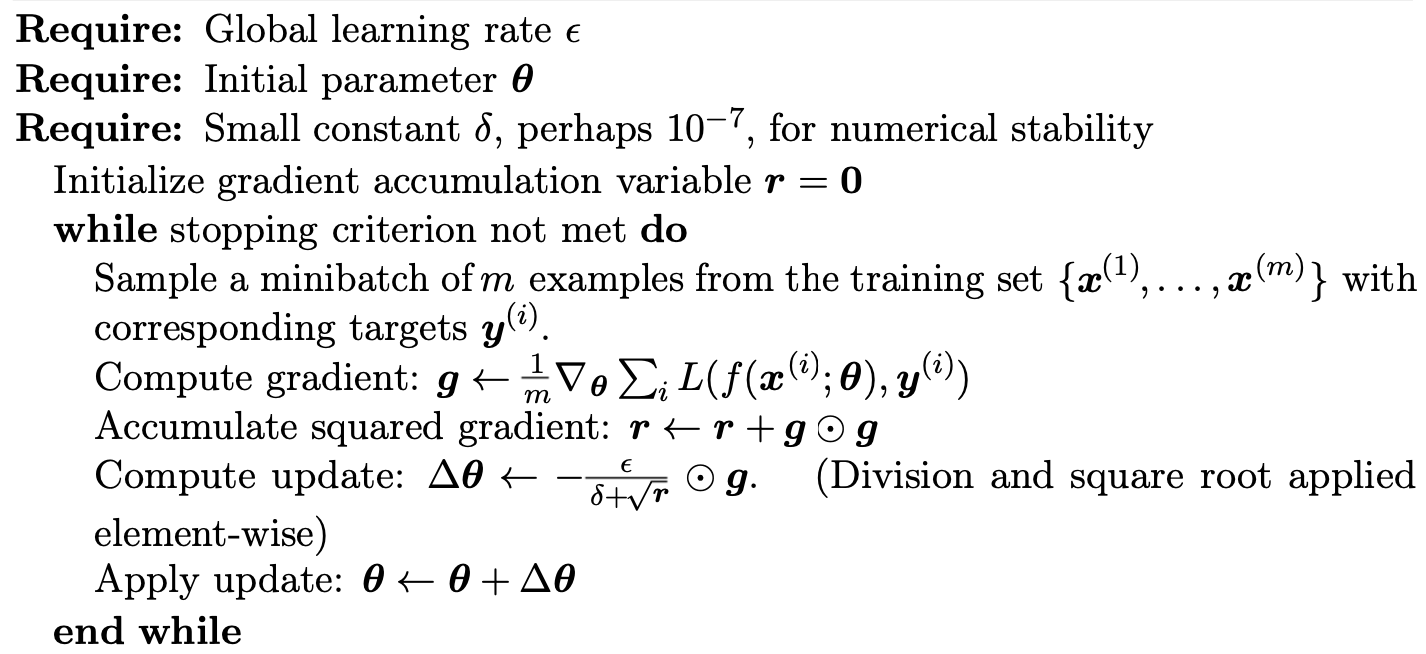
\includegraphics[scale=0.46]{/math/dl/adagrad}
\caption{AdaGrad Algorithm}
\end{figure}

\begin{remark} \hlt{AdaGrad Algorithm}\\
Algorithm individually adapts learning rates of all model parameters by scaling them inversely proportional to square root of sum of all of their historical squared values. Has greater progress in more gently sloped directions of parameter space. On deep neural networks, accumulation of squared gradients from beginning of training can result in premature and excessive decrease in effective learning rate.
\end{remark}

\begin{figure}[H]
\centering
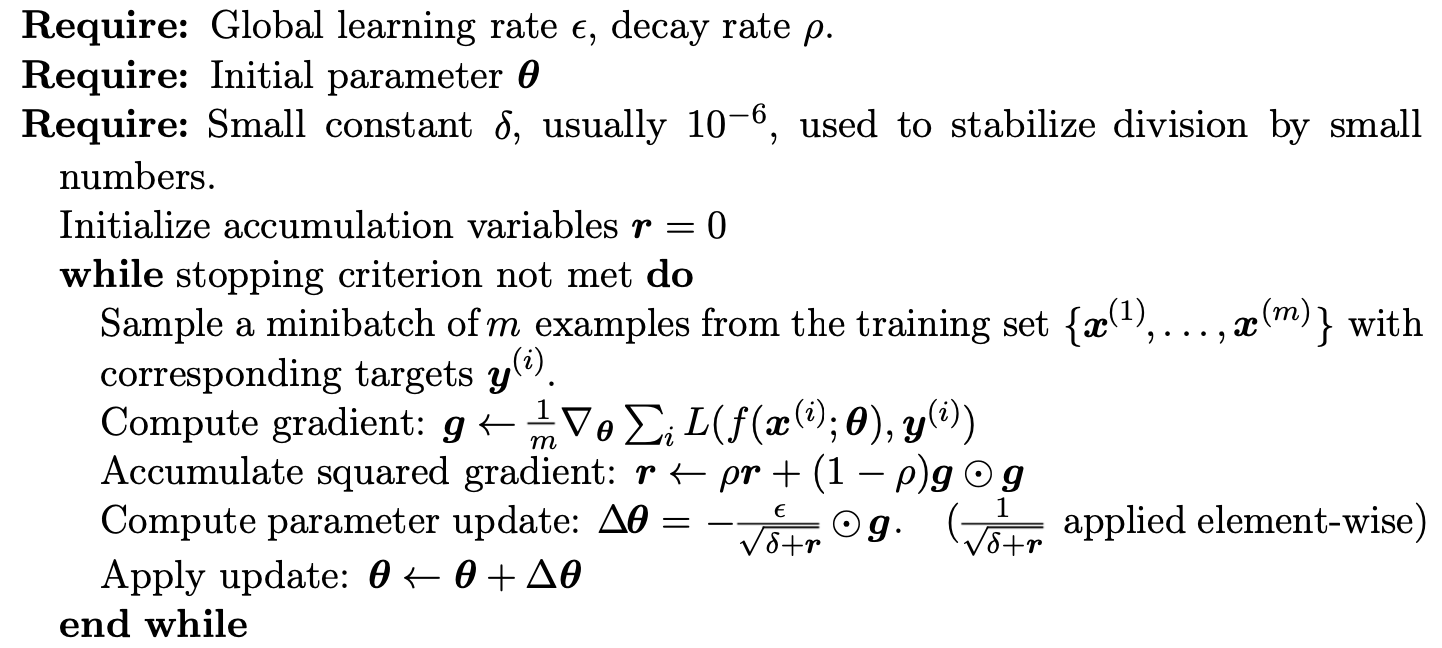
\includegraphics[scale=0.46]{/math/dl/rmsprop}
\caption{RMSPorp Algorithm}
\end{figure}

\begin{figure}[H]
\centering
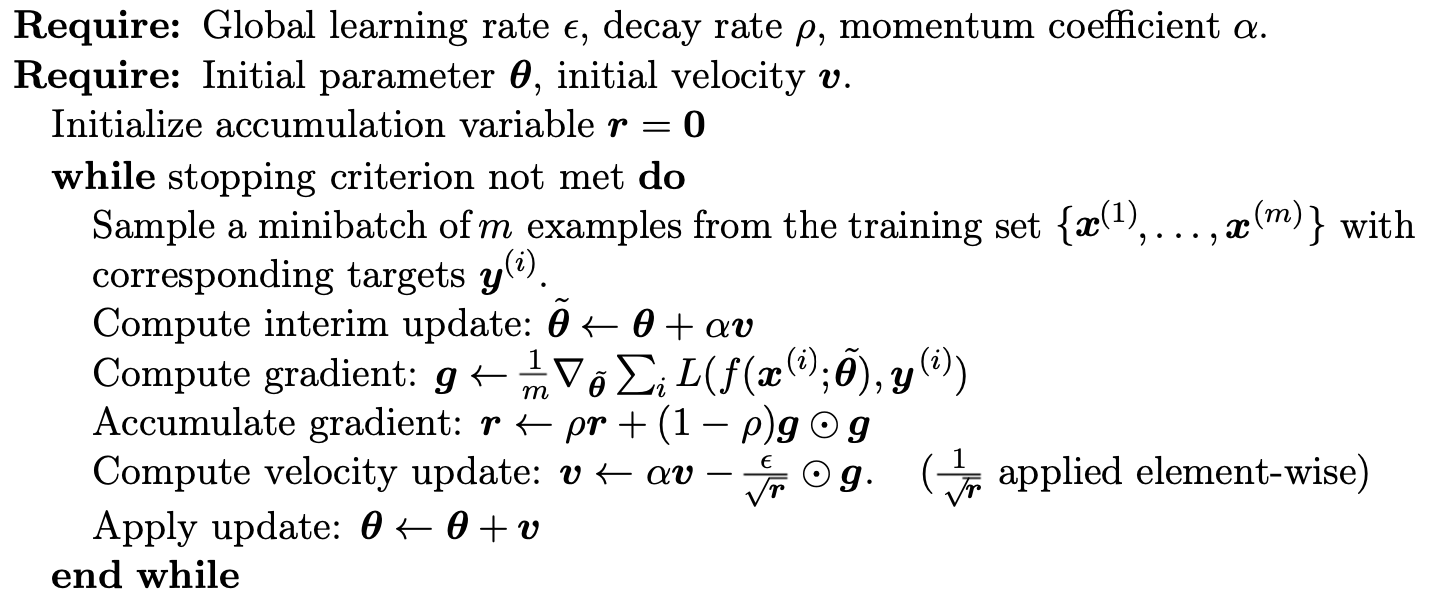
\includegraphics[scale=0.45]{/math/dl/rmspropnest}
\caption{RMSPorp Algorithm with Nesterov momentum}
\end{figure}

\begin{remark} \hlt{RMSProp Algorithm}\\
Modifies AdaGrad to perform better in non-convex setting by changing gradient accumulation into exponentially weighted moving average. RMSProp is effective and practical for deep neural networks.
\end{remark}

\begin{figure}[H]
\centering
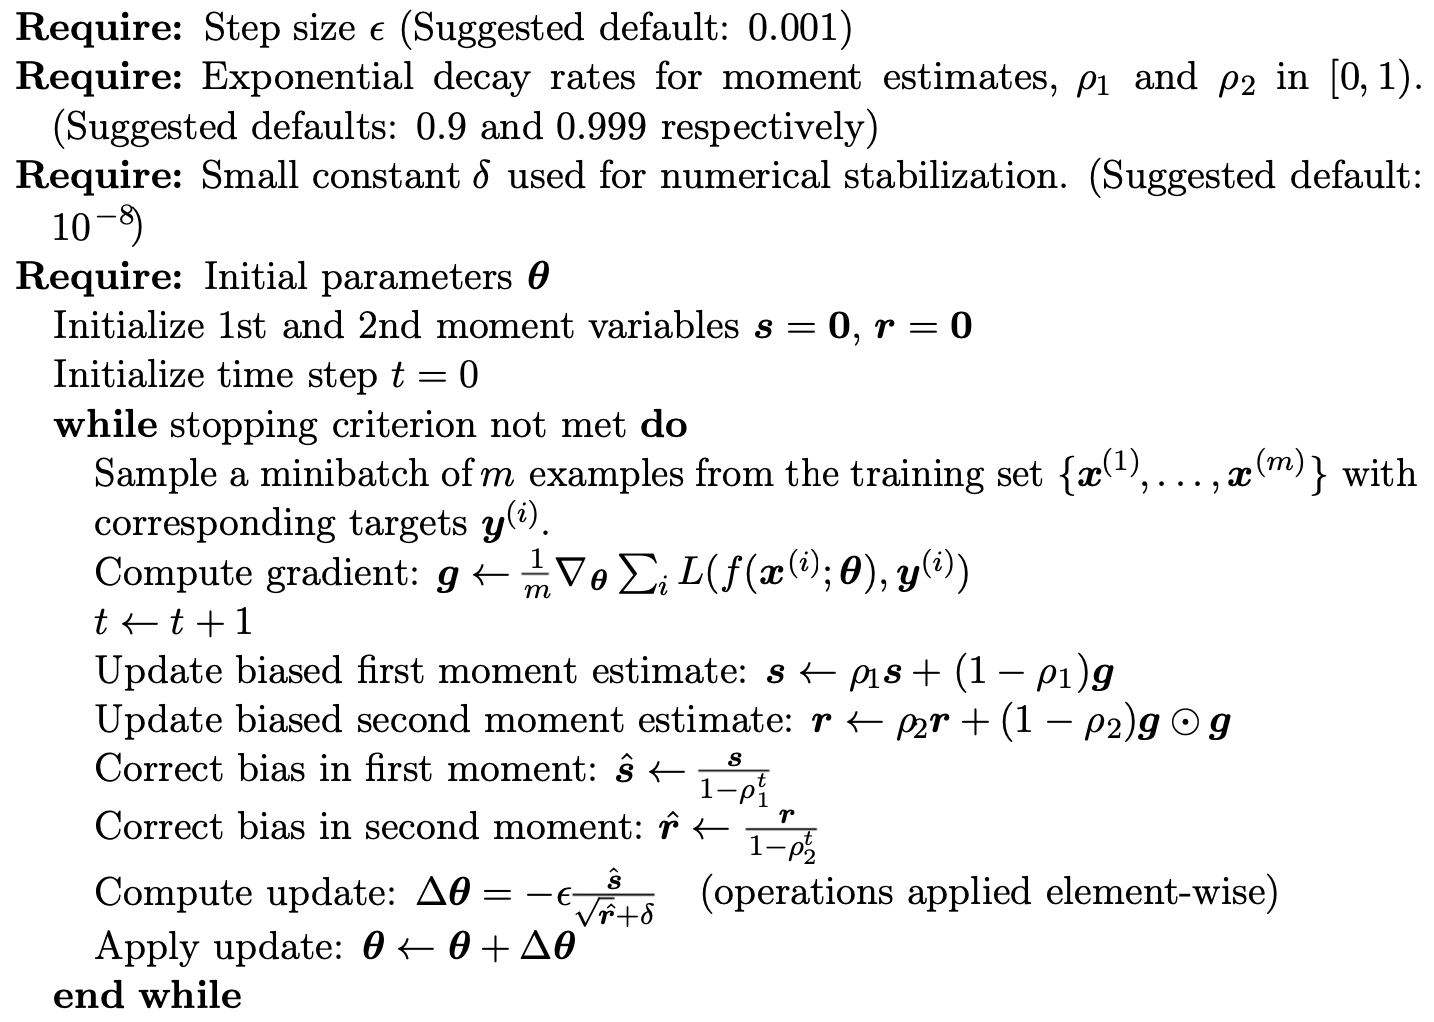
\includegraphics[scale=0.45]{/math/dl/adam}
\caption{Adam Algorithm}
\end{figure}

\begin{remark} \hlt{Adam Algorithm}\\
Variant on combination of RMSProp and momentum. Note, momentum is incorporated directly as an estimate of first order moment of gradient; bias corrections are made to estimates of both first-order moments and second-order moments to account for initialisation at origin.\\
Algorithm is fairly robust to choice of hyper-parameters.
\end{remark}
